\section{Experimental Setup.} \label{cap:ExpSetup}

One ADA and one ADC pads were tested, these pads are identical to the modules 
in the experiment, except for the fibres lengths (47 cm in the tested modules). 
Both fibre bundles were coupled to a PMT and for the readout we used an 
electronic system identical to the one installed in ALICE \cite{Zoccarato}. %
For the beam test the pads were labeled as AD1 and AD2 for ADA and ADC 
respectively. In addition two scintillator counters and two Cherenkov  
radiators were used during the beam test. %The hodoscopes were also used to trigger cosmics.
\\
%\subsection{T10 beam line.}
To study the performance of AD under controlled conditions we used the 
facilities from T10 \cite{t10BeamArea} which delivers secondary particles, 
mainly pions ($\pi^{+}$) and protons ($p^{+}$) produced in the Protron 
Synchrotron (PS) machine \cite{Simon:PS,psBeam}. It is possible to adjust the 
parameters from the beam such like: momentum of the particles, beam size spot 
and beam focus. For the beam test we use four different momentum values: 1.0, 
1.5, 2.0 and 6 GeV/c, with a resolution of 1.3\%.

%\subsection{Experimental setup configurations.}
The setup consists of two different configurations, one used to measure cosmic 
rays and another for particles from T10 beam. In both cases the nominal 
voltages were fixed to 1650 and 1500 Volts for AD1 and AD2 respectively.
The first setup was placed in order to obtain the MIP position with cosmic rays
\cite{cosmicsAD}, two scintillator counters, labeled as \textit{Black-start}  
and \textit{Black-end}, were placed above and below of AD1 and AD2. The setup 
for the beam test in T10 is shown in Figure \ref{figure:BeamSetup}. %
The arrangement is labeled in the beam direction, indicated by the red arrow, 
and corresponds to: Two scintillator counters, Black-start and Black-end 
separated by a distance of 1221 cm and two Cherenkov radiators (provided by T0 
detector group) labelled as \textit{T0-start} and \textit{T0-end}.
%
To readout the signals from all detectors we used a standalone system identical to the Data Acquisition installed in the experiment \cite{ADNote}. 
%\input{NIM-tex/redoutElectronic1.tex}
%
%\subsubsection{Trigger.}\label{subsection:trigger}   
Is important to point out that the data acquisition was triggered by define a logical \texttt{AND} either by the scintillator counters or T0 detectors. The signals passes for a preamplifier that split the signal in to two, one amplified by ten and another by one, that are used by the Front End Electronics (FEE \cite{Zoccarato}) to measure time and charge respectively.
%When the pulse amplified by a factor of 10 crosses the threshold level it generates a leading edge  trigger, in our case the threshold level was fixed to $-40$ mV. 
%\input{NIM-tex/trigger.tex}
\begin{figure}[ht!]
	\begin{center}
		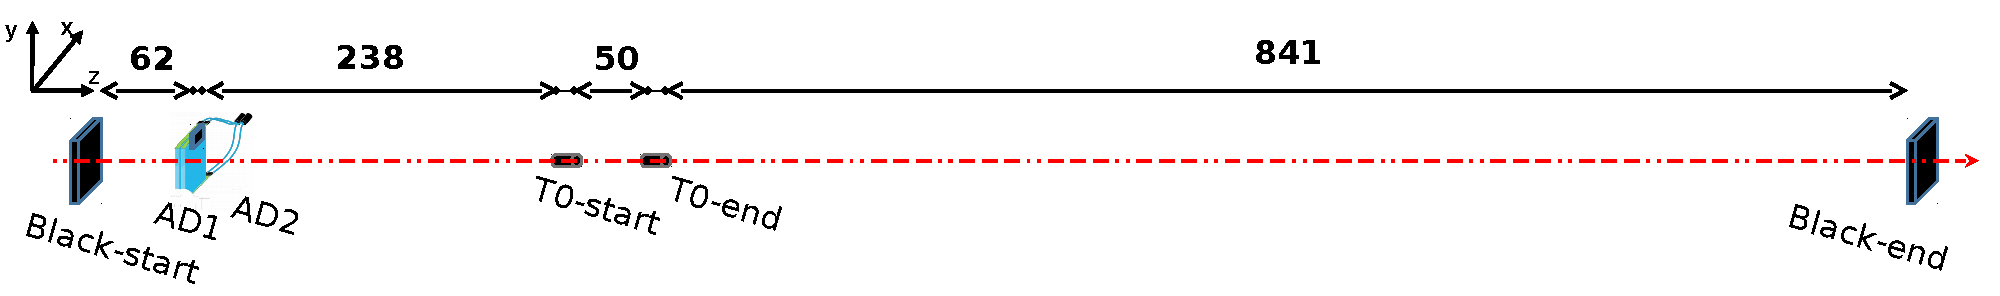
\includegraphics[scale=0.44]{images/BeamTest-Setup_v4.pdf}
		\caption{
		Beam test setup in the T10 beam line. The beam direction goes from 
		left to right. All distances are given in centimeters.
		}
		\label{figure:BeamSetup}
	\end{center}
\end{figure}
%\input{NIM-tex/setup_conf.tex}